\chapter{Introduction}
For years, researchers have turned to methods such as bio-mimicry to ... {\color{red} complete this intro thing}

\section{Background to the study}
The UCT mechatronics laboratory's Rapid Acceleration and Manoeuvrability group studies cheetahs with the aim of reproducing their extraordinary manoeuvrability in two and four legged robots. For this, they require footage of cheetahs as they run. The cameras must be placed in pairs to achieve depth perception. {\color{red} (cite)}

The researchers currently place multiple static cameras, each pair covering a different area, in order to continuously film an animal as it moves around. An illustration of this can be seen in Figure~\ref{fig:multiple_gopro_pairs}. \\

% TODO: cite picture from change.org 'add cheetah emoji' petition?
\begin{figure}[h!]
  \centering
  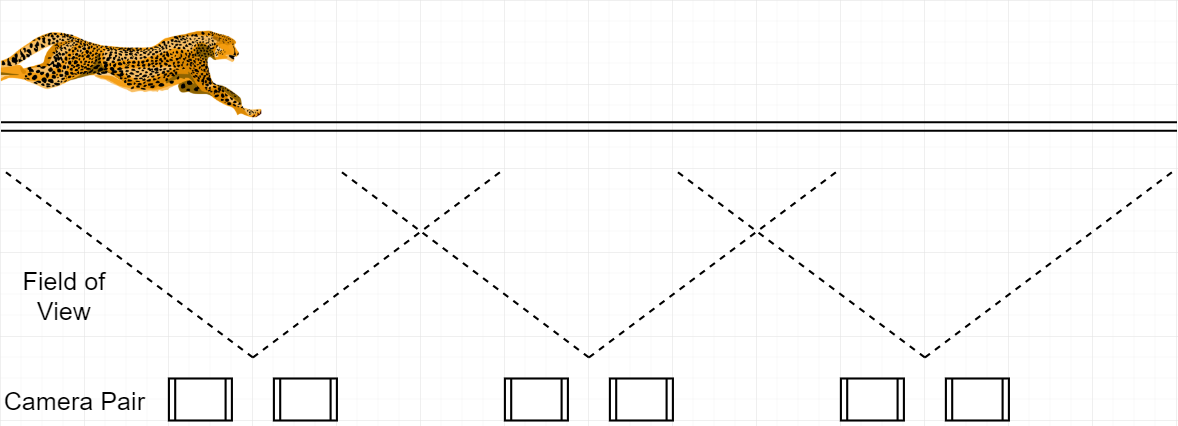
\includegraphics[width=\textwidth]{multiple_gopro_pairs}
  \caption{\label{fig:multiple_gopro_pairs} An illustration of the camera set up in a typical animal movement study.}
\end{figure}

Unfortunately, this setup is not without its disadvantages. Having multiple cameras requires significant amounts of setup time, effort into synchronizing the footage, money spent on cameras and extra work in keeping all cameras recharged. In addition, to maximise the time spent recording the animal, the cameras are usually set to wide-angle mode. This introduces distortion into the recordings. {\color{red} (cite)}

This results in the following question: what if the cameras could instead rotate to track the cheetah as it moves? This way, only a single pair of cameras would be required. An illustration of this in two moments of time is shown in Figure~\ref{fig:single_gopro_pair}.

\begin{figure}[h!]
  \centering
  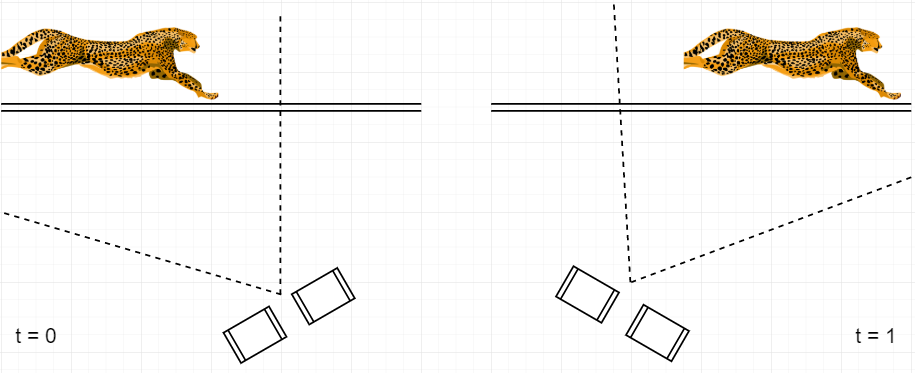
\includegraphics[width=\textwidth]{single_gopro_pair}
  \caption{\label{fig:single_gopro_pair} The proposed solution: a single pair of cameras tracking an animal as it moves.}
\end{figure}

In order to not disturb the animal, it is desired to keep the tracked object free of any sensor equipment. {\color{red} stop here or keep going an properly introduce the idea of using computer vision, etc?}

\section{Objectives of the study}
Based on the aforementioned scenario, the objective of the study is to design, build and test a system which can autonomously identify and track a fast-moving object using modern computer vision methods. A successful design would be able to rotate a pair of cameras to continuously aim at an object, track the object for longer, and not require the cameras to be set to distorting wide-angle modes.

Note that, while the ability to autonomously track an object has a wide range of applications, it is useful to limit oneself to a particular need in order to produce quantifiable 'success or failure' metrics. Thus, this project and report will mainly be about solving a specific issue, with the premise that the project can be used for other applications with minimal modification. Discussions on literature and other applications will treat the system as a general object tracker.


\section{Scope and limitations}
Due to the limited time and finances in an undergraduate thesis, the system will not be tested on actual cheetahs during the course of the project. Instead, it will be tested on humans in complex environments with the hope that this sufficiently mimics the scenario of tracking cheetahs (or any other fast-moving object, for that matter).

However, the neural network will be retrained to be able to track cheetahs. This will be tested in simulation.

Finally, the study will be limited to tracking only one object in the frame at a time. This is because it is not immediately obvious what should be done when more than one object is present in the frame.


\section{Plan of development}
The development schedule was as follows:

\begin{enumerate}
\item Design the structure of the system as a whole.
\item Set up the main computing platform (a raspberry pi), installing relevant software and testing the camera module.
\item Choose a neural network architecture and deploy it onto a neural accelerator stick.
\item Design and 3D print a camera gimbal, and procure the necessary controller and actuators.
\item Rewrite the gimbal controller communication standard in python to allow the raspberry pi to send and receive commands.
\item Model the expected movement of the tracked object, and then design and implement a Kalman Filter.
\item Implement a parallel process-based data pipeline which takes a photo on the picam, preprocessess it, passes it through the neural accelerator, retrieves the results, passes the results into the Kalman Filter and then commands the gimbal motors to re-orient the camera appropriately.
\item Test final the system.
\item Write a report which summarizes the entire project.
\end{enumerate}

\section{Report outline}

The report begins with a review of the current literature surrounding object tracking. As the system combines a number of technologies, it also presents previous knowledge on all of the components which ultimately formed a part of final system.

Next, a more detailed description of the problem, plan of action, activities and project timeline are provided.

Following that are a few chapters which discuss the actual methodology used in the design and implementation of the tracking system. This is done with the aim that reproducing and extending the project can be done with minimal effort.

The results of testing the system are then shown.

Finally, the report ends off with conclusions on the project's success or failure, along with recommendations for future work.
